% tikzpic.tex
\documentclass[crop,tikz]{standalone}%
\usepackage{xcolor}
\colorlet{lightred}{red!50}
\colorlet{lightblue}{blue!50}
%\usetikzlibrary{...}% tikz package already loaded by 'tikz' option
\begin{document}
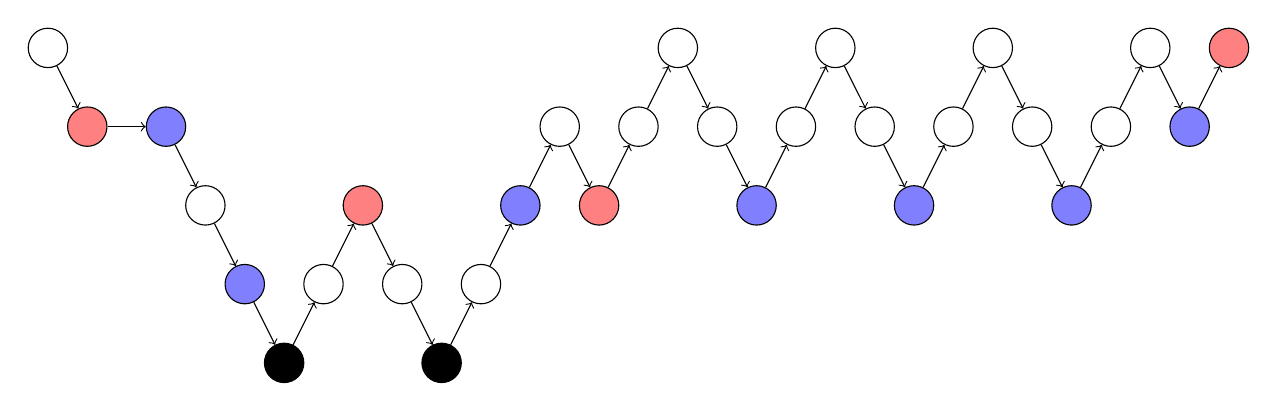
\begin{tikzpicture}
	\node	(a) at (0,4) [draw, circle,inner sep=0pt,minimum size=5mm] {\phantom{\tiny 1.00}};
	\node	(b) at (0.5,3) [draw, circle,fill=lightred,inner sep=0pt,minimum size=5mm] {\phantom{\tiny 1.00}};
	\node	(c) at (1.5,3) [draw, circle,fill=lightblue,inner sep=0pt,minimum size=5mm] {\phantom{\tiny 1.00}};
	\node	(d) at (2,2) [draw, circle,inner sep=0pt,minimum size=5mm] {\phantom{\tiny 1.00}};
	\node	(e) at (2.5,1) [draw, circle,fill=lightblue,inner sep=0pt,minimum size=5mm] {\phantom{\tiny 1.00}};
	\node	(f) at (3,0) [draw, fill=black,circle,inner sep=0pt,minimum size=5mm] {\phantom{\tiny 1.00}};
	\node	(g) at (3.5,1) [draw, circle,inner sep=0pt,minimum size=5mm] {\phantom{\tiny 1.00}};
	\node	(h) at (4,2) [draw, circle,fill=lightred,inner sep=0pt,minimum size=5mm] {\phantom{\tiny 1.00}};
	\node	(i) at (4.5,1) [draw, circle,inner sep=0pt,minimum size=5mm] {\phantom{\tiny 1.00}};
	\node	(j) at (5,0) [draw, circle,fill=black,inner sep=0pt,minimum size=5mm] {\phantom{\tiny 1.00}};
	\node	(k) at (5.5,1) [draw, circle,inner sep=0pt,minimum size=5mm] {\phantom{\tiny 1.00}};
	\node	(l) at (6,2) [draw, circle,fill=lightblue,inner sep=0pt,minimum size=5mm] {\phantom{\tiny 1.00}};
	\node	(m) at (6.5,3) [draw, circle, inner sep=0pt,minimum size=5mm] {\phantom{\tiny 1.00}};
	\node	(n) at (7,2) [draw, circle,fill=lightred, inner sep=0pt,minimum size=5mm] {\phantom{\tiny 1.00}};
	\node	(o) at (7.5,3) [draw, circle, inner sep=0pt,minimum size=5mm] {\phantom{\tiny 1.00}};
	\node	(p) at (8,4) [draw, circle, inner sep=0pt,minimum size=5mm] {\phantom{\tiny 1.00}};
	\node	(q) at (8.5,3) [draw, circle, inner sep=0pt,minimum size=5mm] {\phantom{\tiny 1.00}};
	\node	(r) at (9,2) [draw, circle, fill=lightblue, inner sep=0pt,minimum size=5mm] {\phantom{\tiny 1.00}};
	\node	(s) at (9.5,3) [draw, circle, inner sep=0pt,minimum size=5mm] {\phantom{\tiny 1.00}};
	\node	(t) at (10,4) [draw, circle, inner sep=0pt,minimum size=5mm] {\phantom{\tiny 1.00}};
	\node	(u) at (10.5,3) [draw, circle, inner sep=0pt,minimum size=5mm] {\phantom{\tiny 1.00}};
	\node	(v) at (11,2) [draw, circle, fill=lightblue, inner sep=0pt,minimum size=5mm] {\phantom{\tiny 1.00}};
	\node	(w) at (11.5,3) [draw, circle, inner sep=0pt,minimum size=5mm] {\phantom{\tiny 1.00}};
	\node	(x) at (12,4) [draw, circle, inner sep=0pt,minimum size=5mm] {\phantom{\tiny 1.00}};
	\node	(y) at (12.5,3) [draw, circle, inner sep=0pt,minimum size=5mm] {\phantom{\tiny 1.00}};
	\node	(z) at (13,2) [draw, circle, fill=lightblue, inner sep=0pt,minimum size=5mm] {\phantom{\tiny 1.00}};
	\node	(aa) at (13.5,3) [draw, circle, inner sep=0pt,minimum size=5mm] {\phantom{\tiny 1.00}};
	\node	(bb) at (14,4) [draw, circle, inner sep=0pt,minimum size=5mm] {\phantom{\tiny 1.00}};
	\node	(cc) at (14.5,3) [draw, circle, fill=lightblue, inner sep=0pt,minimum size=5mm] {\phantom{\tiny 1.00}};
	\node	(dd) at (15,4) [draw, circle, fill=lightred, inner sep=0pt,minimum size=5mm] {\phantom{\tiny 1.00}};
	\draw 
	(a) edge[->] (b) 
	(b) edge[->] (c)
	(c) edge[->] (d)
	(d) edge[->] (e)   
	(e) edge[->] (f)
	(f) edge[->] (g)
	(g) edge[->] (h)
	(h) edge[->] (i)
	(i) edge[->] (j) 
	(j) edge[->] (k)
	(k) edge[->] (l)
	(l) edge[->] (m)   
	(m) edge[->] (n)
	(n) edge[->] (o)
	(o) edge[->] (p)
	(p) edge[->] (q)
	(q) edge[->] (r)
	(r) edge[->] (s)
	(s) edge[->] (t)
	(t) edge[->] (u)
	(u) edge[->] (v)
	(v) edge[->] (w)
	(w) edge[->] (x)
	(x) edge[->] (y)
	(y) edge[->] (z)
	(z) edge[->] (aa)
	(aa) edge[->] (bb)
	(bb) edge[->] (cc)
	(cc) edge[->] (dd)
	;
\end{tikzpicture}

\end{document}